\documentclass[thesis.tex]{subfiles}
\begin{document}

\chapter{Comparative genomics}
\label{ch:comparative}

Outline ideas:
\begin{itemize}
  \item Introduction / overview:
  \begin{itemize}
    \item The use of models in PC (very brief)
    \item Specific models used in PC, with strong focus on the most common (KPC), and derivates.  Cover ease-of-use briefly.
    \item Current knowledge re: how appropriate the models are.  Consider histology, genetic features, disease progress (incl. metastatic potential), response to therapy.  Highlight gap in genetic information, and relevance to response to therapy.
    \item Brief overview of known genetic features of human disease.  Raise possibility of subtypes.
    \item Wrap-up with overview of project:
    \begin{enumerate}
      \item Collect matched tumour-normal DNA from a range of GEMMs.
      \item Sequence and determine conserved model-specific and general patterns of somatic mutation.
      \item Compare observed patterns to human disease.
      \begin{itemize}
        \item Are genetic features of human disease recapitulated generally in the models?
        \item Does a single model match the genetic features of human disease much better than the others?
        \item Do specific models serve as simulations of certain subtypes of human disease?
      \end{itemize}
    \end{enumerate}
    \item Overall thesis for this work: \\
    Matching patterns of genetic alterations in mouse models of pancreatic cancer to those seen in human disease can inform researchers as to which models are generally best, and which best match specific patient types. \\
    Sub-theses:
    \begin{itemize}
      \item The patterns of mutations seen in common mouse models of pancreatic cancer match those consistently seen in human disease.
      \item Different mouse models possess different mutation spectra, and models may be close fits to specific genetic subtypes of patients.
    \end{itemize}
  \end{itemize}
  
  \item Results
  \begin{enumerate}
    \item Somatic SNV and indels
    \item CNV and LOH
  \end{enumerate}

  \item Conclusion
  
\end{itemize}

\section{Methods}

\subsection{Models}

\subsection{Sample Origin and Processing}

\subsection{Sequencing}

\subsection{QC}

\subsection{Mapping}

For initial mapping, all lanes were processed independently.  SHRiMP was used to map colourspace reads to the mm10 genome using `all-contigs' and `single-best-mapping' options.  Unpaired reads in the source fastq files were mapped as single reads; paired reads were mapped with pair mode `opp-in', and a per-fastq insert size distribution estimated from a normal distribution fit to insert sizes of the first 10,000 reads.  Likely duplicate reads were marked using Picard MarkDuplicates on each individual lane \gls{BAM}, using an optical duplicate pixel distance parameter of 10.

Lane \glspl{BAM} were progressively merged: first, duplicate lane \glspl{BAM} for a given mouse and sample type (tumour or normal) were combined, then tumour and normal \glspl{BAM} for a given mouse, and finally combined tumour-normal \glspl{BAM} for all mice.  Prior to each level of merging, the \gls{GATK} was used to separately perform \gls{LABQSR} on each input \gls{BAM}.  Finally, the full experiment \gls{BAM} file was recalibrated with \gls{LABQSR}, and then split by mouse and sample type for analysis, yielding 62 paired tumour and normal final \glspl{BAM}.

\subsection{Somatic SNV and Indel Detection}

muTect and Strelka were used separately to detect somatic \glspl{SNV} and \glspl{indel} in individual mouse tumour and normal \glspl{BAM}.  muTect was supplied default parameters; Strelka used the parameter settings given in listing \ref{lst:comp_strelka_settings}; these are the default parameters as recommended for use with the BWA mapper, with the exception that in this work isSkipDepthFilters was set to 1.

\begin{lstlisting}[caption=Strelka configuration file used for SNV / indel detection,label=lst:comp_strelka_settings]
[user]
isSkipDepthFilters = 1
maxInputDepth = 10000
depthFilterMultiple = 3.0
snvMaxFilteredBasecallFrac = 0.4
snvMaxSpanningDeletionFrac = 0.75
indelMaxRefRepeat = 8
indelMaxWindowFilteredBasecallFrac = 0.3
indelMaxIntHpolLength = 14
ssnvPrior = 0.000001
sindelPrior = 0.000001
ssnvNoise = 0.0000005
sindelNoise = 0.000001
ssnvNoiseStrandBiasFrac = 0.5
minTier1Mapq = 20
minTier2Mapq = 5
ssnvQuality_LowerBound = 15
sindelQuality_LowerBound = 30
isWriteRealignedBam = 0
binSize = 25000000
\end{lstlisting}


\subsection{CNV and LOH Detection}

Overview:
\begin{itemize}
  \item Very brief background of CNV and LOH in tumours, and the possibility of detection from NGS data.  Maybe pull in the hallmarks paper, or perhaps specific PC / GEMM examples.
  \item Brief overview of existing techniques and why unsuited?
  \begin{itemize}
    \item CNV:
    \begin{itemize}
      \item Exome pulldown complication
      \item Ill-posed nature of problem
      \item Human-specific methods
      \item Outbred population-specific methods
    \end{itemize}
    \item LOH:
    \begin{itemize}
      \item That Bayesian thing.  Unfortunately affected by CNV, which is unknown.
    \end{itemize}
  \end{itemize}
  \item LOH:
  \begin{itemize}
    \item Maths linking diploid and bias to observed fractions.
    \item Use of FET / similar to detect deviation
    \item HMM on P-value mixture distibution for FDR control and calling.
  \end{itemize}
  \item CNV:
  \begin{itemize}
    \item Ideal maths and assumptions.
    \item Simplifications: Multinomial \--> Poisson \--> Normal
    \item Implementation under Fisherian approach.
    \item HMM on P-values as before, using 3 mixes based on symmetry of statistic.
  \end{itemize} 
\end{itemize}


\subsubsection{Loss of heterozygosity at individual loci}

This work took a simple approach to identify loci with significant evidence of \gls{LOH} in a tumour sample: locate high-confidence heterozygous loci in matched normal DNA, and then test only these heterozygous loci for a significant change in allelic fraction between matched tumour and normal samples.

Location of high-confidence heterozygous loci in normal DNA was achieved using samtools mpileup, and a custom filter based on Bayes factors (algorithm \ref{alg:comp_find_het}).  samtools mpileup provides, per locus, posterior log-likelihoods for each possible genotype, $\ell(G = g|D) = \log(P(D|G = g))$, where $D$ are the observed read data at the locus, and $g$ is a genotype.  These genotype likelihoods for each of the two possible genotype classes, homozygous and heterozygous, must be combined 

\begin{eqnarray}
Hom & = & \{AA, CC, GG, TT\} \\
Het & = & \{AC, AG, AT, CG, CT, GT\}
\label{eq:comm_het_genotypes}
\end{eqnarray}

\begin{eqnarray}
K & = & \frac{P(D|G \in Het)}{P(D|G \in Hom)} \\
  & = & \frac{\sum_{g \in Het} P(D|G = g)P(G = g|G \in Het) }{\sum_{g \in Hom} P(D|G = g)P(G = g|G \in Hom) }
\label{eq:comm_het_bayes}
\end{eqnarray}

\begin{equation}
K = \frac{\frac{1}{|Het|}\sum_{g \in Het} P(D|G = g)}{\frac{1}{|Hom|}\sum_{g \in Hom} P(D|G = g) }
\end{equation}

\begin{algorithm}
  \KwData{Total sequence depth at the locus $D$, minimum depth for call $mindepth$, list of alternate alleles $A$, list of Phred-scaled genotype likelihoods $L$, minimum likelihood difference in bits between top two genotypes $mindelta$, minimum Bayes factor in bits for heterozygous to be called over homozygous $minscore$.}
  \KwResult{A boolean: true if the locus is called heterozygous, false if it is not}

  \Begin {
    \If {$D \leq mindepth$}{
      \KwRet false\;
    }
    \tcp{Convert Phred-scaled likelihoods to nats}
    \For{$i \leftarrow 1$ \KwTo $|L|$}{
      $L_i \longleftarrow -0.23025851 L_i$\;
    }
    \tcp{Ensure the likelihood difference between the two most likely genotypes is at least $mindelta$.  The 1.442695 factor converts bits to nats.}
    $L^* \longleftarrow L$ sorted in decreasing order\;
    \If {$L^*_1 - L^*_2 \le mindelta \div 1.442695$}{
      \KwRet false\;
    }
    \tcp{Calculate combined likelihoods for heterozygous and homozygous genotypes}
    \Switch{$|A|$}{
      \Case{$2$}{
        $L_{het} \longleftarrow L_2$\;
        $L_{hom} \longleftarrow \log\left(\frac{1}{2}\sum_{i \in \{1, 3\}} \exp(L_i) \right)$\;
      }
      \Case{$3$}{
        $L_{het} \longleftarrow \log\left(\frac{1}{6}\sum_{i \in \{2, 4, 5, 7, 8, 9\}} \exp(L_i) \right)$\;
        $L_{hom} \longleftarrow \log\left(\frac{1}{4}\sum_{i \in \{1, 3, 6, 10\}} \exp(L_i) \right)$\;
      }
      \Case{default}{
        \KwRet false\;
      }
    }

  \tcp{Compute the Bayes factor for heterozygous vs homozygous, and compare to the threshold}
  \If {$L_{het} - L_{hom} \le minscore \div 1.442695$}{
    \KwRet false\;
  }
  
  \KwRet true\;
  
  }
  \label{alg:comp_find_het}
  \caption{Determine if a locus is heterozygous}
\end{algorithm}

\subsubsection{Copy number variation at individual loci}



\subsubsection{Combining calls from adjacent loci}

\Gls{CNV} and \gls{LOH} are broad genomic events that typically affect many adjacent loci together, yet the methods presented in the preceding sections consider each locus in isolation.  By examining loci separately, we disregard important information: that the \gls{CNV} and \gls{LOH} status of nearby loci is strongly correlated.  Intuitively, by leveraging these local correlations and combining results from neighbouring loci, we can achieve more accurate \gls{CNV} and \gls{LOH} detection than if each locus were considered alone.

A number of approaches could be used to smooth LOH and CNV calls and share information between neighbouring loci; in this work I chose the \gls{HMM} formalism and extended the Pounds-Morris FDR estimator\cite{Pounds2003} to the locality-sensitive case.  The Pounds-Morris procedure fits the observed distribution of test P-values to a mixture of Uniform and Beta distributions.  The Uniform distribution models the expected distribution of P-values under the null hypothesis, whereas the Beta distribution approximately fits the highly left-skewed distribution of P-values expected of tests for which the null hypothesis is false.  After the observed distribution of P-values has been fit to the Beta-Uniform mixture model, the \gls{FDR} associated with a given P-value can be estimated from the densities of the Beta and Uniform component distributions at that P-value.

The original Pounds-Morris procedure considers all tests as equivalent, and thus integrates no locality information, but for the \gls{LOH} case combining the procedure with the locality-sensitive \gls{HMM} is straightforward (figure~\ref{fig:comp_loh_hmm}).  The \gls{HMM} moves between two discrete states: \emph{No LOH}, and \emph{LOH}.  The \emph{No LOH} state emits a Uniform distribution of P-values, as expected under the null hypothesis of no \gls{LOH}, whereas the \emph{LOH} state emits a left-skewed Beta distribution of P-values, approximating the P-value distribution observed for loci at which the null hypothesis is false.  Observed P-values at a chain of adjacent loci are fit to the \gls{HMM} by standard algorithms, and the posterior probability of a locus being in state \emph{No LOH} directly gives the locality-adjusted \gls{FDR} for that locus.  In cases where too few extreme P-values are present to reliably estimate the parameters of the Beta distribution, the fit becomes unstable and \gls{FDR} estimates potentially unreliable.  To handle this situation gracefully, the method fits both the full \emph{No LOH / LOH} model, and a restricted \emph{No LOH} only model, and selects the model with the superior \gls{BIC}.

\begin{figure}
\centering
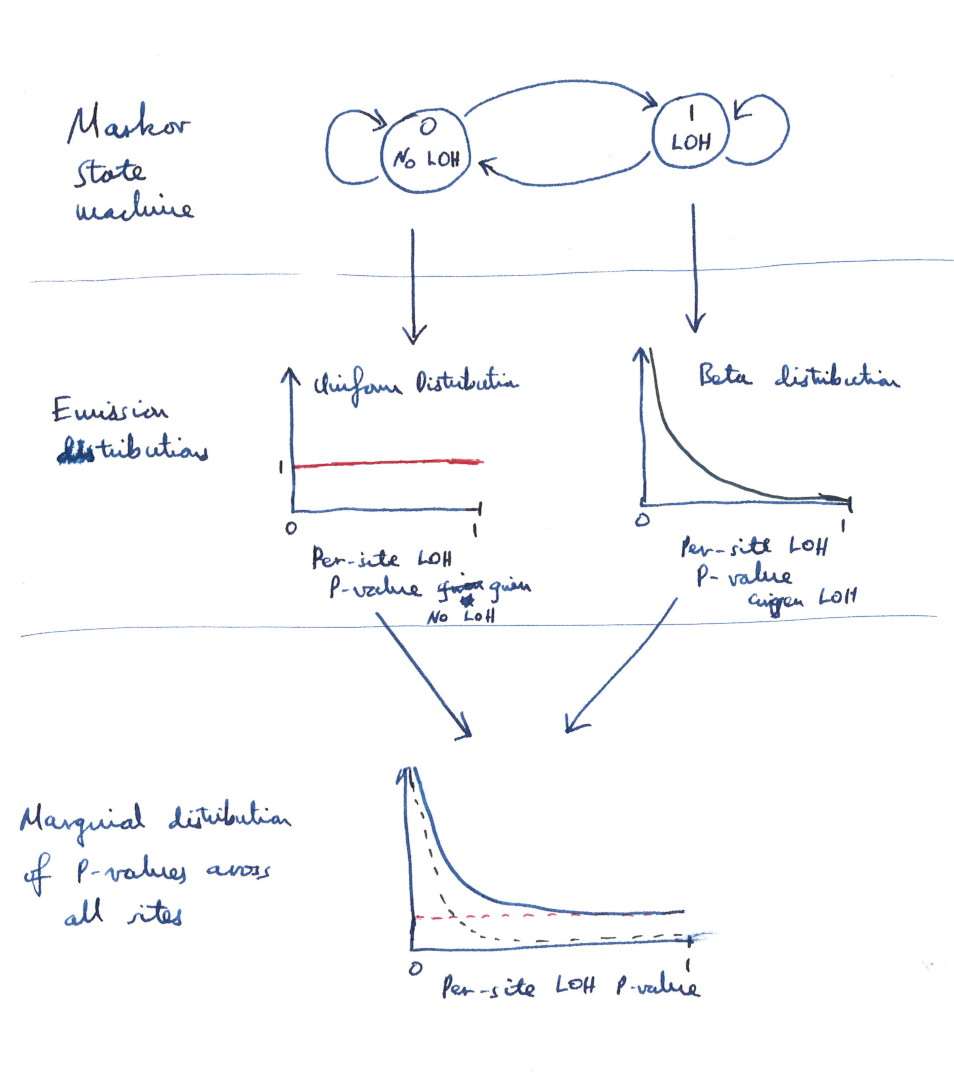
\includegraphics[width=100mm]{resources/comp_loh_hmm.jpg}
\caption{Locality-sensitive FDR estimation of LOH calls using a Markov chain Beta-Uniform mixture model.\label{fig:comp_loh_hmm}}
\end{figure}

Extension of the procedure to the \gls{CNV} case requires three states: \emph{Diploid}, \emph{Loss}, and \emph{Gain} (figure~\ref{fig:comp_cnv_hmm}).  The \emph{Loss} and \emph{Gain} states are modelled by Beta distributions, left-skewed in the \emph{Loss} case, and right-skewed in the \emph{Gain} case.  The posterior probability of a locus being in state \emph{Diploid} then gives the overall \gls{FDR} for a \gls{CNV} call at that locus.  \Gls{BIC} model selection is performed as for the \gls{LOH} case, except in this case four models are compared: \emph{Diploid}, \emph{Diploid / Loss}, \emph{Diploid / Gain}, and \emph{Loss / Diploid / Gain}.

\begin{figure}
\centering
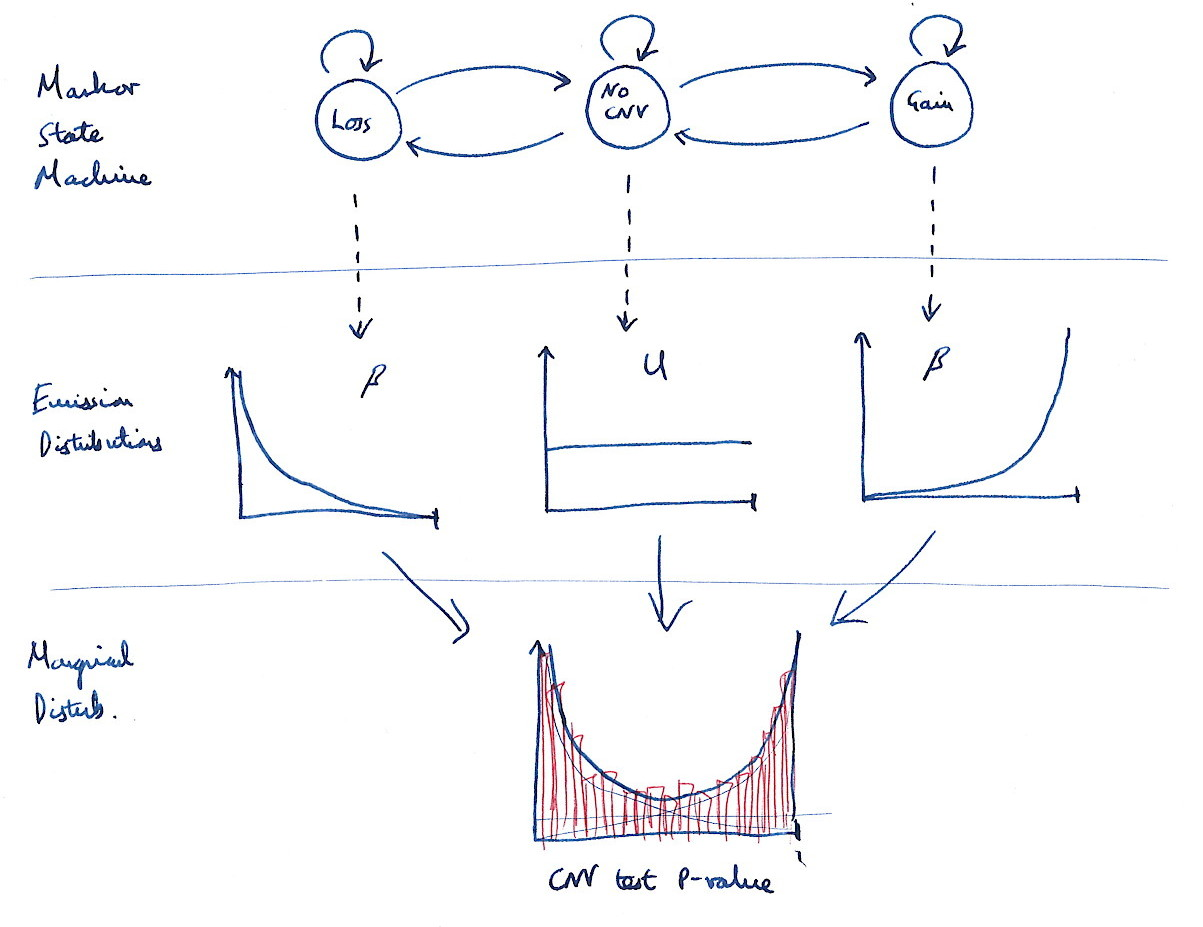
\includegraphics[width=100mm]{resources/comp_cnv_hmm.jpg}
\caption{Locality-sensitive FDR estimation of CNV calls using a Markov chain double-Beta-Uniform mixture model.\label{fig:comp_cnv_hmm}}
\end{figure}

Although the given procedure is simple in formulation, some additional complexities were required for a practical implementation, all related to the high degree of flexibility of the Beta distribution.  The Uniform distribution is a special case of the Beta distribution, and therefore in cases where the distribution of P-values is near Uniform (ie. all sites appear to satisfy the null hypothesis), the fitting problem is ill-posed.  This issue was resolved by enforcing $\alpha \leq 0.95$ for \gls{LOH} and \gls{CNV} loss detection, and $\beta \leq 0.95$ for \gls{CNV} gain detection.  For \gls{FDR} correction of \gls{CNV} P-values, structural zeros were placed on the probabilities of direct transitions between \emph{Loss} and \emph{Gain} states (figure \ref{fig:comp_cnv_hmm}); although such transitions are biologically plausible, they were found to contribute to unstable fits in noisy data.

%\bibliographystyle{plain}
%\bibliography{thesis}

\end{document}
